\documentclass[12pt]{article}

\usepackage{pablo}
\usepackage{multicol}

\usepackage[a4paper,margin=0.9cm]{geometry}

\pagestyle{empty}

\begin{document}

\begin{center}
  Algorithmique --- Probabilités

  {\large
    \textsc{Marche aléatoire}
  }

  ------------------
\end{center}

Une tortue se trouve au centre d'un carré de 10 pas de côté. Elle avance en faisant chaque pas au hasard dans une des quatre directions (gauche, droite, haut, bas). On se demande au bout de combien de pas, en moyenne, elle va sortir du carré.

On désigne par $P$ le nombre de pas nécessaires pour sortir du carré. Ce n'est pas un nombre « fixe » : il dépend de l'expérience (comme le résultat du lancé d'un dé) ; c'est ce qu'on appelle une \emph{variable aléatoire}\footnote{Pas la peine de retenir ce mot : il n'est pas au programme.}.

\section{Étude préliminaire}

\begin{multicols}{2}
On modélise l'expérience en plaçant la tortue à l'origine d'un repère orthonormé, chaque pas correspondant à un déplacement dans une des quatre directions. Un exemple est donné ci-contre.

\begin{enumerate}
  \item Quelle est la plus petite valeur que peut prendre $P$ ?
  \item Montrer que $P$ n'est pas borné, c'est-à-dire que $P$ peut prendre des valeurs aussi grandes que l'on peut imaginer.
  \item Quelle est la probabilité que la tortue sorte par l'arête nord du carré ?
\end{enumerate}

\columnbreak

\begin{center}
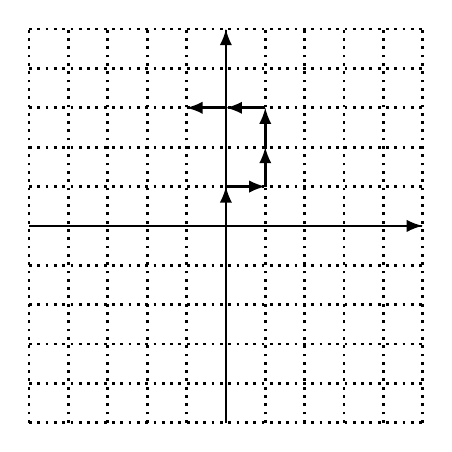
\begin{tikzpicture}[line width=1pt,scale=0.5]
  \draw[dotted](-5,-5) grid (5,5);
  \draw[-latex] (-5,0) -- (5,0);
  \draw[-latex] (0,-5) -- (0,5);

  \draw[-latex] (0,0) -- (0,1);
  \draw[-latex] (0,1) -- (1,1);
  \draw[-latex] (1,1) -- (1,2);
  \draw[-latex] (1,2) -- (1,3);
  \draw[-latex] (1,3) -- (0,3);
  \draw[-latex] (0,3) -- (-1,3);
\end{tikzpicture}
\end{center}
\end{multicols}

\section{Simulation d'une marche}

\begin{enumerate}
  \item Copier le fichier \texttt{marche.py} fourni par le professeur dans
    votre répertoire personnel, et l'exécuter. Que fait-il ?
  \item Comment peut-on tester si la tortue est sortie du carré ? Modifier le
    programme pour qu'il s'arrête lorsque la tortue est sortie (aide : pour
    obtenir l'abscisse et l'ordonnée de la tortue, on pourra utiliser
    \texttt{xcor()} et \texttt{ycor()}).
  \item Modifier le programme pour qu'il compte le nombre de pas, et qu'il
    affiche, à la fin, le nombre de pas effectués par la tortue avant de
    sortir du carré (aide : pour afficher une valeur (par exemple \texttt{n})
    dans la console, on utilise \texttt{print(n)}).
\end{enumerate}

\section{Simulation de plusieurs marches}

On désire maintenant simuler de nombreuses marches, pour pouvoir calculer la
moyenne du nombre de pas nécessaires à la tortue pour sortir du carré.

\begin{enumerate}
  \item Modifier le programme pour qu'il exécute 4 fois de suite la
    simulation (aide : on pourra utiliser la fonction \texttt{restart()}, qui
    permet de réinitialiser le programme).
  \item Ajouter juste après les lignes \texttt{import} la ligne suivante.
    Elle permet de faire avancer la tortue plus vite, et de ne pas dessiner
    tous ses déplacements, ce qui accélère la simulation.

    \texttt{tracer(100, 0)}
  \item Réaliser 100 simulations au lieu de 4.
  \item Modifier le programme pour qu'il calcule la moyenne du nombre de pas
    faits par la tortue avant de sortir du carré.
\end{enumerate}



\end{document}
